% =============================================================================
% Chapitre — Le marché marocain : ce que vingt ans de données changent
%
% Aucun chiffre de ce chapitre n'est saisi à la main. Les grandeurs de panel et
% de performance proviennent de data/gold/deep_morocco_results.json et
% deep_morocco_estimand_family.json ; les grandeurs de puissance proviennent de
% docs/EVALUATION_LIMITS.md §5 et de la section CORRECTION 2026-09-15 de
% docs/DEEP_MOROCCO_EXPERIMENT.md, elles-mêmes recalculées dans
% notebooks/phase11_statistical_power_and_overfitting.ipynb.
%
% Ce chapitre existe parce que l'étude marocaine profonde était auparavant
% réduite à une ligne du tableau « cinq pistes fermées » du chapitre 5. C'est
% l'expérience la plus directement liée au terrain du projet, et la seule qui
% réponde à la question « et si le problème était simplement le manque
% d'historique marocain ? ».
% =============================================================================

\chapter{Le marché marocain : ce que vingt ans de données changent}
\label{chap:maroc}

Le chapitre précédent se termine sur un constat négatif~: sur les univers
publiés, aucune couche d'apprentissage n'établit d'avantage face à son
comparateur. Ce constat admet deux lectures, et elles n'ont pas les mêmes
conséquences. Ce chapitre construit le dispositif qui permet de les départager,
sur le terrain qui intéresse le plus l'entreprise d'accueil~: la Bourse de
Casablanca.

% =============================================================================
\section{Deux lectures d'un même résultat}
% =============================================================================

La première lecture est que le signal est \emph{absent}~: le marché est
suffisamment efficient pour qu'une prédiction de rendement par apprentissage
n'apporte rien d'exploitable. La seconde est que le signal a été
\emph{affamé}~: l'univers \texttt{full\_2021} ne compte que neuf actifs et
environ 11\,700 lignes de panel, et la fenêtre de test gelée couvre moins de
deux ans. Avec si peu d'observations, un effet réel mais modeste ne peut tout
simplement pas être détecté.

Ces deux lectures produisent le même verdict statistique et appellent des
décisions opposées. La première clôt le sujet. La seconde désigne un remède
précis~: davantage de données. Elle a l'avantage d'être testable, et c'est ce
test que décrit ce chapitre.

\begin{remarquebox}
La question posée n'est donc pas « le modèle est-il bon~? » mais « le dispositif
d'évaluation avait-il les moyens de le dire~? ». C'est une question sur la
\emph{puissance} du protocole, pas sur la qualité du modèle.
\end{remarquebox}

% =============================================================================
\section{Constituer vingt ans de Bourse de Casablanca}
% =============================================================================

\subsection{Ce que les sources permettent réellement}

La contrainte qui fixe le début de l'univers canonique à juillet 2021 n'est pas
un choix~: c'est la profondeur de la source gratuite utilisée pour la BVC. La
recherche de données plus anciennes a établi deux faits.

Aucune \textbf{interface programmatique gratuite} ne dessert l'historique
antérieur à 2021 des valeurs de Casablanca~: les identifiants \texttt{.CS} sont
absents des fournisseurs usuels — seul Maroc Telecom est accessible, et
seulement via sa cotation croisée à Euronext Paris — et le candidat payant
abordable examiné ne couvre pas la place de Casablanca. En revanche, un
fournisseur de données de marché grand public propose le \textbf{téléchargement
manuel} de l'historique quotidien de chaque valeur depuis son introduction, avec
un plafond de 5\,000~lignes par fichier.

Le 22~juillet~2026, les historiques quotidiens de \textbf{17~valeurs cotées à
Casablanca}, ainsi que l'indice MASI, ont été téléchargés par cette voie. Les
fichiers bruts sont conservés dans la couche Bronze, hors dépôt Git comme
l'ensemble des données.

\subsection{L'univers retenu}

Des 17~valeurs, l'univers \textsc{profond} retient les \textbf{12~titres à
historique continu depuis 2005}, choisis sur ce seul critère et non sur leur
performance. Ils couvrent la banque (ATW, BCP, CIH, BOA), les
télécommunications (IAM), le ciment (LHM, CMA), les mines (MNG), la sidérurgie
(SID), la consommation (CSR), l'énergie (GAZ) et l'assurance (WAA)~: la
structure sectorielle réelle de la cote casablancaise.

\begin{table}[htbp]
  \centering
  \caption[Univers canonique et panel marocain profond]{Ce que l'extension
  change, en volume de données et en couverture historique.}
  \label{tab:maroc-univers}
  \small
  \begin{tabular}{lrr}
    \toprule
     & Univers canonique & Panel profond \\
     & \texttt{full\_2021} & \textsc{deep} \\
    \midrule
    Actifs                          & 9        & \textbf{12} \\
    Historique                      & 2021-07 $\rightarrow$ 2026 & \textbf{2005-01 $\rightarrow$ 2024-05} \\
    Séances                         & ---      & 4\,682 \\
    Lignes de panel                 & $\approx$ 11\,700 & \textbf{56\,184} ($\approx \times 5$) \\
    Fenêtre de test hors échantillon & $\approx$ 1,7~an & \textbf{6,75~ans} \\
    Contient la crise de 2008        & non      & \textbf{oui} \\
    \bottomrule
  \end{tabular}
\end{table}

\subsection{Ce que ces données ne sont pas}

Trois réserves sont consignées ici plutôt que laissées à découvrir, car elles
déterminent le statut du résultat.

Les prix sont des \textbf{cours de clôture non ajustés} en dirhams~: ni les
dividendes ni les divisions d'actions n'y sont réintégrés. C'est une limite
réelle pour une mise en production — le chapitre~\ref{chap:architecture} montre
combien le traitement du dividende pèse sur une performance mesurée — mais elle
n'affecte pas la question posée ici, qui porte sur la \emph{capacité
prédictive} d'un classement transversal et non sur un rendement total.

Le plafond de 5\,000~lignes \textbf{tronque les historiques les plus anciens}~:
la fenêtre assemblée s'arrête en mai~2024. Le raccordement avec la source
récente, dont les périodes se recouvrent entre 2021 et 2024, est un travail
d'industrialisation, non nécessaire pour répondre à la question.

Enfin, les \textbf{calendriers de cotation} diffèrent légèrement d'un fichier à
l'autre~; ils sont alignés sur un calendrier de jours ouvrés de référence avec
report avant borné, exactement comme la chaîne traite déjà les données BVC
canoniques.

% =============================================================================
\section{Le protocole : celui du chapitre 4, sans adaptation}
% =============================================================================

Pour que la comparaison ait un sens, la machinerie d'évaluation honnête décrite
au chapitre~\ref{chap:modelisation} est réutilisée \emph{sans modification}~:
changer à la fois les données et la règle du jeu n'aurait rien établi.

\textbf{Étape A — la mesure directe, sans portefeuille.} Validation croisée
par blocs purgés avec embargo, les hyperparamètres des forêts aléatoires et du
gradient boosting étant choisis sur le \emph{coefficient d'information}. Cette
étape ne suppose aucun coût de transaction et ne construit aucune allocation~:
elle mesure la compétence prédictive seule, ce qui est exactement ce qu'il faut
pour savoir si le modèle était sous-alimenté.

\begin{definitionbox}{Coefficient d'information (IC)}
Le \emph{coefficient d'information} est la corrélation de rang entre les
rendements prédits et les rendements effectivement réalisés à la période
suivante. Il vaut $0$ quand le classement prédit n'a aucun rapport avec le
classement réalisé, et $1$ pour un classement parfait. En gestion quantitative
d'actions, un IC de l'ordre de $0{,}05$ est déjà considéré comme exploitable~:
les valeurs utiles sont petites, et c'est leur stabilité qui compte.
\end{definitionbox}

\textbf{Étape B — le test gelé.} Les 35~\% finaux de la période sont réservés
et ne sont ouverts qu'une fois. Les modèles calibrés y sont évalués aux côtés
du système à régimes, de l'équipondéré et des références classiques, chacun
accompagné d'un intervalle de confiance à 90~\% obtenu par bootstrap par blocs.
Les leviers d'allocation sont \textbf{fixés et non sélectionnés} — rétrécissement
à $0{,}5$, pénalité de rotation à $1{,}0$ — précisément pour que cette
expérience réponde à la question des \emph{données} et non à celle du réglage.

% =============================================================================
\section{Étape A — le modèle s'aiguise réellement}
% =============================================================================

Le résultat de l'étape A est net, et il est positif.

\begin{figure}[htbp]
  \centering
  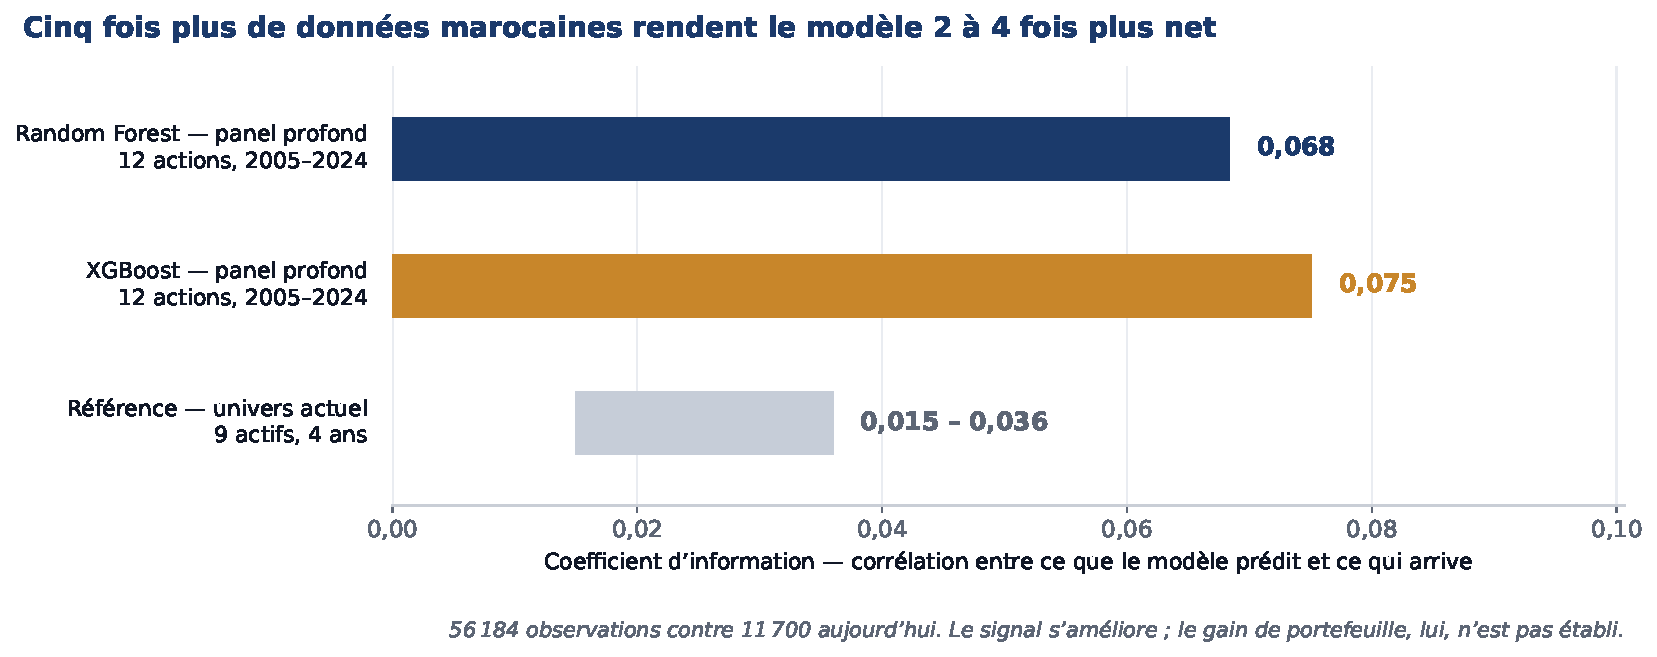
\includegraphics[width=0.92\textwidth]{assets/figures/ic_maroc_profond.pdf}
  \caption[Coefficient d'information : univers canonique et panel profond]{Le
  coefficient d'information mesuré sur le panel marocain profond, comparé à la
  plage obtenue sur l'univers canonique. Les deux familles de modèles
  progressent dans les mêmes proportions.}
  \label{fig:ic-maroc}
\end{figure}

Le coefficient d'information passe de la plage $0{,}015$--$0{,}036$ observée sur
l'univers canonique à \textbf{$0{,}0684$ pour la forêt aléatoire} et
\textbf{$0{,}0751$ pour le gradient boosting}~: une multiplication par un
facteur~2 à~4, obtenue \emph{indépendamment par les deux familles de modèles}.
Cette concordance compte autant que le niveau~: deux algorithmes de nature
différente, entraînés séparément, se déplacent dans les mêmes proportions.

Un IC voisin de $0{,}07$ sort du bruit et entre dans la plage considérée comme
exploitable en gestion transversale d'actions. Sur ce point, la réponse est donc
sans ambiguïté~: \textbf{le signal était, pour partie, affamé}. Davantage
d'historique marocain rend le modèle mesurablement plus fin.

% =============================================================================
\section{Étape B — le portefeuille, lui, ne suit pas}
% =============================================================================

L'étape~B évalue ce que cette finesse devient une fois transformée en
allocation, sur la fenêtre gelée 2017--2024 et nette des coûts de transaction.

\begin{table}[htbp]
  \centering
  \caption[Panel marocain profond : test gelé]{Ratios de Sharpe nets sur la
  fenêtre de test gelée, avec intervalle de confiance à 90~\% par bootstrap
  par blocs. Tous les intervalles contiennent zéro.}
  \label{tab:maroc-sharpe}
  \small
  \begin{tabular}{lrr}
    \toprule
    Stratégie & Sharpe net & IC 90~\% \\
    \midrule
    Forêt aléatoire calibrée   & $0{,}3376$ & $[-0{,}4117~;~+1{,}1399]$ \\
    Équipondéré (1/N)          & $0{,}2525$ & $[-0{,}5570~;~+1{,}1469]$ \\
    Gradient boosting calibré  & $0{,}2238$ & $[-0{,}5053~;~+0{,}9944]$ \\
    Markowitz (Sharpe maximal) & $0{,}1782$ & $[-0{,}5251~;~+0{,}9290]$ \\
    Variance minimale (LW)     & $0{,}1269$ & $[-0{,}5991~;~+0{,}9528]$ \\
    Système à régimes          & $0{,}0669$ & $[-0{,}6467~;~+0{,}8193]$ \\
    \bottomrule
  \end{tabular}
\end{table}

Trois observations s'imposent, et une seule d'entre elles est une conclusion.

D'abord, \textbf{la forêt aléatoire calibrée obtient la meilleure estimation
ponctuelle}, devant l'équipondéré et devant Markowitz. C'est un renversement par
rapport à l'univers canonique, où le système à régimes menait et les challengers
suivaient.

Ensuite, \textbf{tous les intervalles contiennent zéro}, et ils sont larges~: de
l'ordre d'une unité et demie de Sharpe. Aucun écart de ce tableau n'est
établi.

Enfin, et c'est le point le plus instructif, \textbf{le classement s'inverse}
entre les deux univers. Un avantage qui change d'ordre selon l'échantillon est
la signature du bruit, non celle d'un avantage durable. La correction pour le
nombre d'essais confirme cette lecture~: le ratio de Sharpe dégonflé du meilleur
challenger vaut $0{,}6792$ sur les six configurations explorées.

Une procédure de comparaison multiple appliquée à l'ensemble des hypothèses de
cette expérience — 60~hypothèses appariées sur 1\,638~observations — ne retient
\textbf{aucun} survivant au seuil de 5~\%. Aucune stratégie n'est déclarée
supérieure à l'équipondéré.

% =============================================================================
\section{Ce que « pas de gain » signifie exactement}
% =============================================================================

Il serait commode de s'arrêter là et de conclure que davantage de données ne
sert à rien. Ce serait une erreur, et le projet l'a commise avant de la
corriger.

\begin{remarquebox}
La note de recherche initiale affirmait que cette expérience « écarte, preuves à
l'appui, l'idée que davantage d'historique de prix soit le remède ». Cette
affirmation a été \textbf{retirée} lors du réexamen du 15~septembre~2026. Elle
reposait sur des intervalles contenant zéro, ce qui ne dit rien de la capacité
du dispositif à détecter l'effet qu'il cherchait.
\end{remarquebox}

La grandeur qui manquait est l'\textbf{effet minimal détectable}~: le plus petit
écart que le protocole repère huit fois sur dix, au seuil retenu. Comparer
l'écart observé à cet effet minimal indique si le dispositif avait, ou non, les
moyens de conclure.

\begin{figure}[htbp]
  \centering
  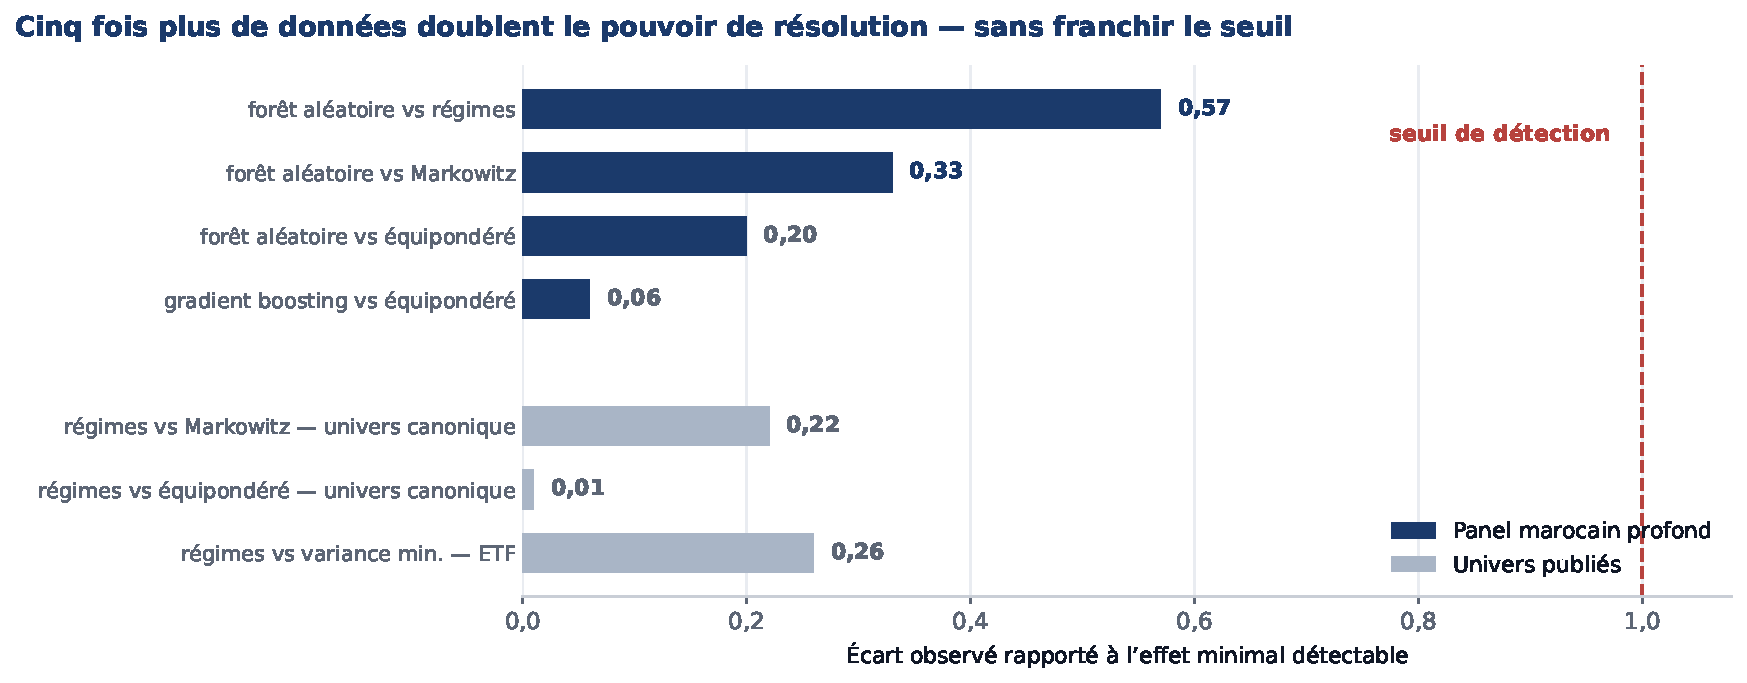
\includegraphics[width=0.92\textwidth]{assets/figures/puissance_maroc.pdf}
  \caption[Pouvoir de résolution du protocole]{Écart observé rapporté à l'effet
  minimal détectable. Une barre atteignant $1{,}0$ correspond à un dispositif
  tout juste capable de trancher~; en deçà, le verdict négatif est déterminé par
  la taille de l'échantillon avant tout ajustement de modèle.}
  \label{fig:puissance-maroc}
\end{figure}

Sur l'univers canonique, ce rapport se situe entre $0{,}01$ et $0{,}26$~: le
verdict négatif y était \textbf{inscrit dans le dispositif} avant qu'aucun
modèle ne soit ajusté. Sur la fenêtre gelée, l'écart détectable atteint
$0{,}765$, soit environ sept fois le plus grand écart réellement observé~; à
effet constant, il faudrait de l'ordre de 12\,000~séances — près de
quarante-huit ans — pour que ce protocole puisse départager les deux stratégies.

Sur le panel marocain profond, le même rapport atteint \textbf{$0{,}57$} pour la
comparaison entre la forêt aléatoire calibrée et le système à régimes. Autrement
dit, cinq fois plus de données n'ont pas « échoué à aider »~: elles ont
\textbf{plus que doublé le pouvoir de résolution} du dispositif. Elles ne l'ont
simplement pas porté jusqu'au seuil. À effet observé constant, franchir ce seuil
demanderait environ $3{,}1$~fois plus d'observations hors échantillon, soit de
l'ordre de 5\,045~séances — une vingtaine d'années supplémentaires.

\begin{resultatbox}{La distinction qui porte tout ce chapitre}
« N'a pas franchi le seuil » et « est écarté » sont deux énoncés différents, et
seul le premier est soutenu par cette expérience. Le résultat n'autorise pas à
conclure que davantage de données marocaines serait inutile~; il quantifie, au
contraire, ce qu'il en faudrait.
\end{resultatbox}

% =============================================================================
\section{Ce qui ne s'est pas reproduit}
% =============================================================================

Le réexamen du 15~septembre~2026 a rejoué l'expérience depuis les fichiers
bruts, avec le même script. L'univers se reconstruit à l'identique~:
12~valeurs~$\times$~4\,682~séances, du 6~janvier~2005 au 31~mai~2024, sans
valeur manquante. Les coefficients d'information se reproduisent, de même que
les ratios de Sharpe de l'équipondéré, de Markowitz et du système à régimes.

\textbf{Celui du gradient boosting ne se reproduit pas.} Il ressort à
$0{,}2238$ contre $0{,}28$ lors de la campagne initiale. L'écart suffit à
renverser un énoncé qualitatif~: à $0{,}2238$, le gradient boosting calibré
passe \emph{sous} l'équipondéré, et l'affirmation « les stratégies
d'apprentissage obtiennent les meilleures estimations ponctuelles » ne vaut plus
que pour la forêt aléatoire. La cause la plus probable est une dérive de version
de la bibliothèque de gradient boosting entre les deux exécutions.

Cette hypothèse ne peut pas être confirmée, et c'est en soi un enseignement~:
ni les fichiers bruts ni le panel assemblé ne sont empreintés par une somme de
contrôle. Un artefact d'entrée haché aurait permis de trancher entre dérive de
bibliothèque et dérive de données. C'est une lacune de traçabilité, nommée ici
au même titre que les autres, et la première chose à corriger si ce panel doit
être industrialisé.

% =============================================================================
\section{Ce qu'il faudrait pour intégrer ce panel à la release}
% =============================================================================

Ce panel reste une \textbf{expérience de recherche}. Il n'alimente ni l'API, ni
le tableau de bord, ni aucun résultat publié au chapitre~\ref{chap:resultats}.
Cinq chantiers le séparent d'un statut de release, et ils sont d'ingénierie de
données bien plus que de modélisation~:

\begin{itemize}
  \item \textbf{Réconcilier les sources} — raccorder l'historique profond à la
        source récente sur leur période de recouvrement 2021--2024, et vérifier
        que le raccord ne crée ni saut de prix ni doublon.
  \item \textbf{Réintégrer les dividendes} à leur date de détachement, et traiter
        les opérations sur titres (divisions, attributions).
  \item \textbf{Contractualiser la source} — les droits de redistribution d'un
        téléchargement manuel ne sont pas ceux d'un flux sous contrat.
  \item \textbf{Empreinter les entrées} par une somme de contrôle, pour que la
        non-reproductibilité observée plus haut devienne diagnosticable.
  \item \textbf{Tenir compte des défauts de mesure propres à la place} — prix
        fréquemment figés et non-synchronicité des séances avec les places
        américaines, dont le chapitre~\ref{chap:global2004} mesure l'ampleur.
\end{itemize}

\begin{resultatbox}{Ce que ce chapitre établit}
Multiplier par cinq l'historique marocain rend le modèle mesurablement plus
fin~: le coefficient d'information est multiplié par un facteur~2 à~4, et les
deux familles de modèles le confirment séparément. Ce gain de précision ne se
transforme pas en avantage de portefeuille établi~: tous les intervalles
contiennent zéro et aucune stratégie ne survit à la comparaison multiple. Mais
le dispositif a plus que doublé son pouvoir de résolution, et l'on sait
désormais chiffrer ce qui manque. La limite n'est donc pas la quantité de
données~: c'est la conversion d'une prédictibilité faible mais réelle en un
avantage net de coûts, sur un marché étroit, peu liquide et coûteux à négocier.
\end{resultatbox}
